%Este trabalho está licenciado sob a Licença Atribuição-CompartilhaIgual 4.0 Internacional Creative Commons. Para visualizar uma cópia desta licença, visite http://creativecommons.org/licenses/by-sa/4.0/ ou mande uma carta para Creative Commons, PO Box 1866, Mountain View, CA 94042, USA.

\chapter{Aproximação por mínimos quadrados}\label{cap:ajuste}
\thispagestyle{fancy}

\section{Problemas lineares}\label{sec:problemas_lineares}

Dado um conjunto de $n$ pontos $\{(x_i,y_i)\}_{i=1}^n$, $x_i\neq x_j$ para $i\neq j$, e uma família de $m \leq n$ funções $\{f_i(x)\}_{i=1}^m$, o problema linear de aproximação por mínimos quadrados consiste em determinar os $m$ coeficientes $\{c_i\}_{i=1}^m$ tal que a função
\begin{align}    
  f(x) &= \sum_{i=1}^m c_if_i(x) \\
       &= c_1f_1(x) + c_2f_2(x) + c_3f_3(x) + \cdots + c_nf_n(x)
\end{align}
aproxime o conjunto de pontos dados no sentido de mínimos quadrados, i.e. os coeficientes que são solução do seguinte problema linear de minimização
\begin{equation}\label{eq:pmq}
  \min_{\{c_1,c_2,\dotsc,c_n\}} \sum_{i=1}^n (y_i - f_i(x_i))^2.
\end{equation}

\subsection{Equações normais}

Afim de resolver o problema de mínimos quadrados~\eqref{eq:pmq}, observamos que o erro quadrático
\begin{equation}
  E := \sum_{i=1}^n (y_i - f_i(x_i))^2 = \sum_{i=1}^n \left(y_i - \sum_{j=1}^m c_jf_j(x_i)\right)^2
\end{equation}
tem seu mínimo para os coeficientes $c_k$ tais que
\begin{equation}\label{eq:aux1_mq}
  \frac{\p E}{\p c_k} = 0,\quad k=1, 2, 3, \dotsc, m.
\end{equation}
Calculando estas derivadas parciais, temos
\begin{align}
  \frac{\p E}{\p c_k} &= \frac{\p}{\p c_k} \sum_{i=1}^n \left(y_i - \sum_{j=1}^m c_jf_j(x_i)\right)^2\\
    &= 2\sum_{i=1}^n \left(y_i - \sum_{j=1}^m c_jf_j(x_i)\right)f(x_k)\\
    &= 2\sum_{i=1}^n y_if(x_k) - 2\sum_{i=1}^n\sum_{k=1}^m c_jf_j(x_i)f(x_k),\quad k=1, 2, 3, \dotsc, m.
\end{align}

Desta forma, a equação~\eqref{eq:aux1_mq} é equivalente a resolver o seguinte sistema linear
\begin{equation}\label{eq:aux2_mq}
  \sum_{i=1}^n\sum_{k=1}^m c_jf_j(x_i)f(x_k) = \sum_{i=1}^n y_if(x_k),\quad k=1, 2, 3, \dotsc, m.
\end{equation}

Agora, denotando
\begin{equation}
  A :=
  \begin{bmatrix}
    f_1(x_1) & f_2(x_1) & \cdots & f_m(x_1) \\
    f_1(x_2) & f_2(x_2) & \cdots & f_m(x_2) \\
    \vdots & \vdots & \vdots & \vdots \\
    f_1(x_n) & f_2(x_n) & \cdots & f_m(x_n)
  \end{bmatrix}
\end{equation}
o sistema linear~\eqref{eq:aux2_mq} pode ser escrito na seguinte forma matricial
\begin{equation}\label{eq:equacoes_normais}
  A^TAc= A^Ty,
\end{equation}
onde $c = (c_1, c_2, \dotsc, c_m)$ é o vetor dos coeficientes e $y = (y_1, y_2, \dotsc, y_n)$ é o vetor das abscissas dos pontos dados.

\begin{ex}\normalfont{(Ajuste de polinômios)}\label{ex:ajuste_de_polinomios}
  Considere o problema de ajustar o conjunto de pontos
  \begin{center}
    \begin{tabular}{l|rrrr}
      $i$ & $1$ & $2$ & $3$ & $4$ \\\hline
      $x_i$ & $-1$ & $0$ & $1$ & $1,5$\\
      $y_i$ & $1,2$ & $-0,1$ & $0,7$ & $2,4$\\\hline
    \end{tabular}
  \end{center}
  por um polinômio quadrático da forma
  \begin{equation}
    p(x) = p_1x^2 + p_2x + p_n
  \end{equation}
  no sentido de mínimos quadrados.  

  \begin{figure}[h]
    \centering
    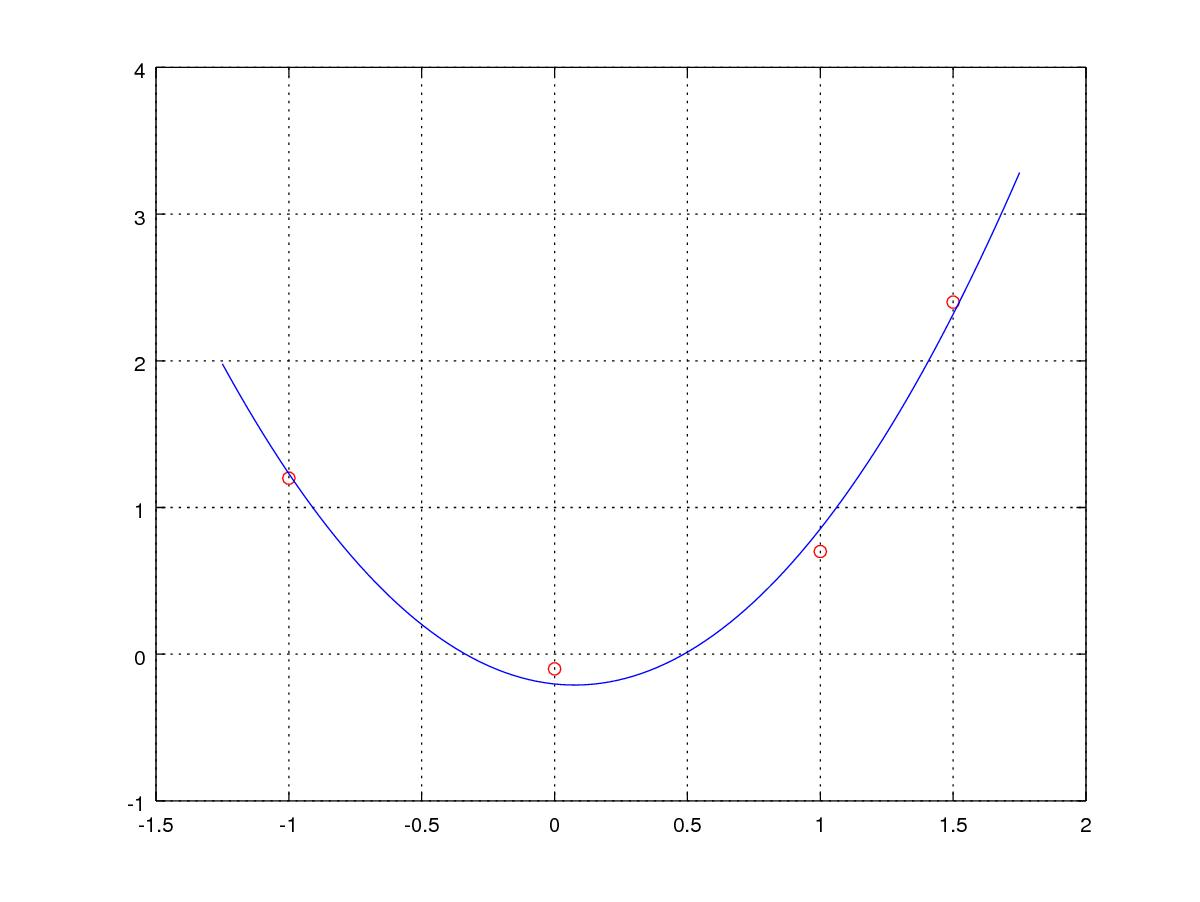
\includegraphics[width=\textwidth]{cap_ajuste/figs/ex_mq_poli/ex_mq_poli}
    \caption{Esboço do polinômio ajustado no Exemplo~\ref{ex:ajuste_de_polinomios}.}
    \label{fig:ex_mq_poli}
  \end{figure}
  
  
  Neste caso, a família de funções do problema de mínimos quadrados é $f_1(x) = x^2$, $f_2(x) = x$ e $f_3(x) = 1$. Assim sendo, os coeficientes $p = (p_1, p_2, p_3)$ são solução do seguinte sistema linear
  \begin{equation}\label{eq:aux3_md}
    A^TAp = A^Ty,
  \end{equation}
  onde $y = (y_1, y_2, y_3)$ e
  \begin{equation}
    A :=
    \begin{bmatrix}
      x_1^2 & x_1 & 1 \\
      x_2^2 & x_2 & 1 \\
      x_3^2 & x_3 & 1 \\
      x_4^2 & x_4 & 1
    \end{bmatrix}.
  \end{equation}
  Emfim, resolvendo as equações normais~\eqref{eq:aux3_md}, obtemos
  \begin{equation}
    p(x) = 1,25x^2 -0,188x - 0,203.
  \end{equation}
  A Figura~\ref{fig:ex_mq_poli} mostra um esboço dos pontos (em vermelho) e do polinômio ajustado (em azul).
  
  \ifisoctave
  Os coeficientes e um esboço do polinômio ajustado podem ser obtidos no \verb+GNU Octave+ com o seguinte código:
\begin{verbatim}
#pontos
x = [-1 0 1 1.5]';
y = [1.2, -0.1, 0.7, 2.4]';

#resol. as eqs. normais
A = [x.^2 x.^1 x.^0];
p = inv(A'*A)*A'*y

#esboco do pol. ajustado
xx = linspace(-1.25,1.75);
plot(x,y,'ro',...
     xx,polyval(p,xx));grid
\end{verbatim}
  \fi
  
\end{ex}


\begin{ex}\normalfont{(Ajuste de curvas)}\label{ex:ajuste_de_curvas}
  Consideremos o mesmo conjunto de pontos do exemplo anterior (Exemplo~\ref{ex:ajuste_de_polinomios}). Aqui, vamos ajustar uma curva da forma
  \begin{equation}
    f(x) = c_1\sen(x) + c_2\cos(x) + c_3
  \end{equation}
no sentido de mínimos quadrados. Para tanto, formamos a matrix
\begin{equation}
  A :=
  \begin{bmatrix}
    \sen(x_1) & \cos(x_1) & 1 \\
    \sen(x_2) & \cos(x_2) & 1 \\
    \sen(x_3) & \cos(x_3) & 1 \\
    \sen(x_4) & \cos(x_4) & 1 \\
  \end{bmatrix}
\end{equation}
  e, então, resolvemos as equações normais $A^TAc = A^Ty$ para o vetor de coeficientes $c=(c_1, c_2)$. Fazendo isso, obtemos $c_1=-0,198$, $c_2=-2,906$ e $c_3=2,662$. A Figura~\ref{fig:ex_mq_curvas} mostra um esboço da curva ajustada (linha azul) aos pontos dados (círculos vermelhos).

  \begin{figure}[h]
    \centering
    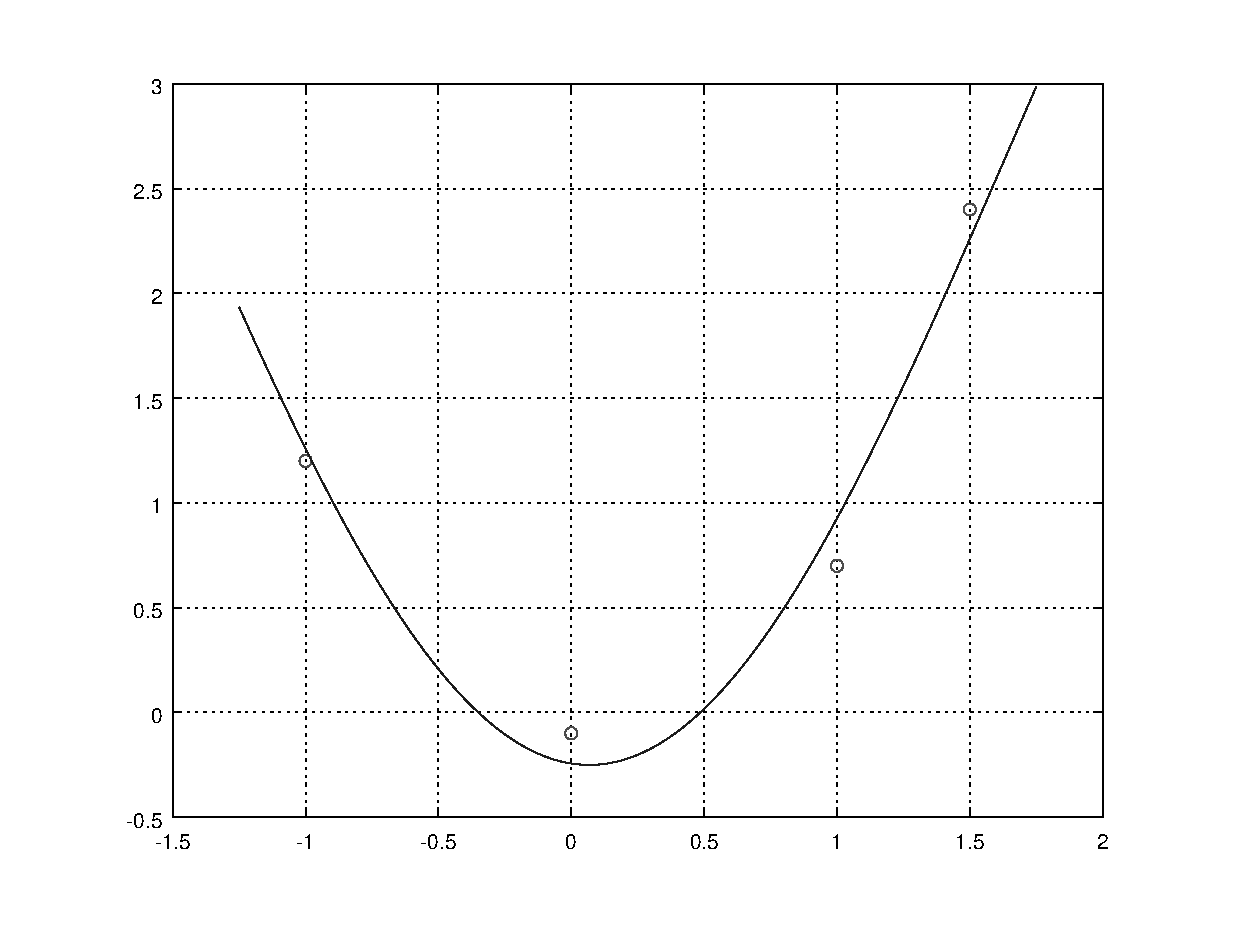
\includegraphics[width=\textwidth]{cap_ajuste/figs/ex_mq_curvas/ex_mq_curvas}
    \caption{Esboço da curva ajustada no Exemplo~\ref{ex:ajuste_de_curvas}.}
    \label{fig:ex_mq_poli}
  \end{figure}

\ifisoctave
Os coeficientes e um esboço do polinômio ajustado podem ser obtidos no \verb+GNU Octave+ com o seguinte código:
\begin{verbatim}
#pontos
x = [-1 0 1 1.5]';
y = [1.2, -0.1, 0.7, 2.4]';

#resol. as eqs. normais
A = [sin(x) cos(x) ones(4,1)];
c = inv(A'*A)*A'*y

#curva ajustada
f = @(x) c(1)*sin(x) + c(2)*cos(x) + c(3)

#esboco do pol. ajustado
xx = linspace(-1.25,1.75);
plot(x,y,'ro',...
     xx,f(xx));grid
\end{verbatim}
\fi

\end{ex}

% \subsection*{Exercícios}

% \begin{exer}
%   oi
% \end{exer}
% \begin{resp}
%   tchau
% \end{resp}
